\chapter[Deep Networks for Carrier Frequency Offset]{Deep Networks for Carrier Frequency Offset\raisebox{.3\baselineskip}{\normalsize\footnotemark}}
\footnotetext{The contents of this chapter were produced in collaboration with Nikhil Shinde.} 

The carrier frequency offset (CFO) correction process removes the symbol rotation caused by the non-ideal conditions of the transmitter and receiver environment.  We will explore how neural networks can both estimate the CFO and correct for rate of rotation without using backpropagation for each new rate.

\section{Recurrent Neural Network Follows a Circle}

A carrier frequency offset affects the received symbols by slowly rotating them around the origin.  If we want a neural network to be able to correct this, we essentially need it to act as a clock, following around a circle at a certain rate.
We first explore what kind of architectures are necessary for a recurrent neural network (RNN) to learn how to follow a circle.
We show that a simple, small linear RNN can learn to act as the rotation matrix for a single rate of rotation around a circle.
We also show that in order to have an RNN follow a circle for different rates of rotation, we need a large non-linear layer.

\subsection{Single Rate}

Figure~\ref{fig:circle_constant_rate} shows a recurrent neural network (RNN) that follows a circle for a single rate of rotation.  The network's input is the starting point, $x[0]$, and it must predict the next $100$ points, $x[1] \ldots x[99]$.  Point $x[i]$ is rotated by $e^{ij\omega}$ where $\omega$ is the rate of rotation.  The RNN architecture is one linear layer that takes the current point as input, $x[i]$, and outputs the next point, $x[i+1]$.  We are forcing the state of the RNN to be the next point; $\text{state} = x[i+1]$.  We use a linear layer here because the network essentially has to learn how to become the rotation matrix which is linear with respect to the input. 

\begin{align}
R = \begin{bmatrix}
\cos(\omega) & - \sin(\omega) \\
\sin(\omega) & \cos(\omega)
\end{bmatrix}
\end{align} 

\setlength{\tabcolsep}{0pt}
\begin{figure}
  \centering
  \caption{Linear neural network: follow a circle for a constant CFO rate.}
  \begin{tabular}{ccc}
    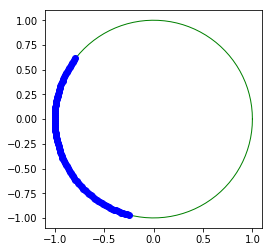
\includegraphics[width=50mm]{figures/cfo/follow_circle_linear_before.png}&
    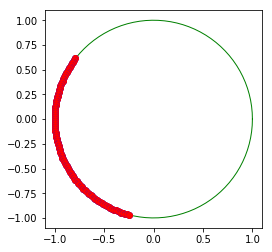
\includegraphics[width=50mm]{figures/cfo/follow_circle_linear_after.png}&
    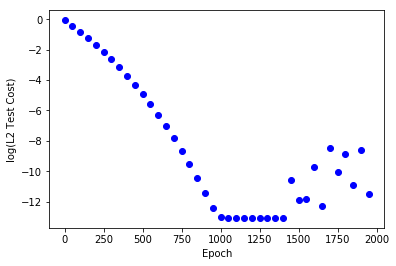
\includegraphics[width=70mm]{figures/cfo/follow_circle_linear_loss.png}\\
  \end{tabular}
  \label{fig:circle_constant_rate}
\end{figure}

The RNN is trained for a constant rate of rotation, $\omega$, applied to sequences of $100$ points.  The network trained for $2k$ epochs, each with a batch size of $1k$ data sequences and with a learning rate of $0.006$.  The initial starting point, $x[0]$ is a uniform random variable drawn from on the unit circle. 
The network is tested on $1k$ new data sequences but with the same $\omega$.
Figure~\ref{fig:circle_constant_rate} shows the results of an RNN trained and tested for $\omega=0.02$.  
The network achieves a loss on the order of $10^{-13}$.  However, the minimum loss is not very sticky.  The network ends up jumping away from this minimum while training.  A more thorough search over learning rate decay is needed to prevent this jumping from happening.

\subsection{Different Rates}


Figure~\ref{fig:circle_diff_rate} shows a recurrent neural network (RNN) that follows a circle for a given rate of rotation.
The network's input is the starting point, $x_0$ and the rate of rotation, $\omega$.
The RNN must predict the next $100$ points, $x_1 \ldots x_{99}$.  Point $x_i$ is rotated by $e^{ij\omega}$.

\setlength{\tabcolsep}{0pt}
\begin{figure}
  \centering
  \caption{Nonlinear neural network: follow a circle for different CFO rates.}
  \begin{tabular}{ccc}
    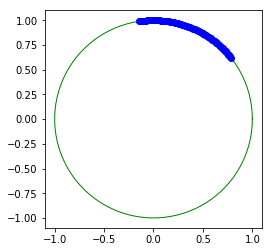
\includegraphics[width=50mm]{figures/cfo/follow_circle_nonlinear_before.png}&
    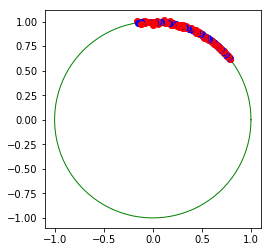
\includegraphics[width=50mm]{figures/cfo/follow_circle_nonlinear_after.png}&
    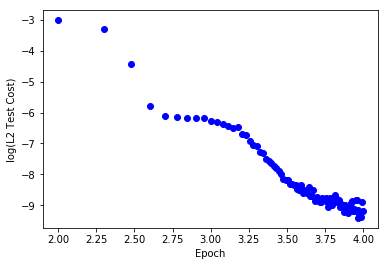
\includegraphics[width=70mm]{figures/cfo/follow_circle_nonlinear_loss.png}\\
  \end{tabular}
  \label{fig:circle_diff_rate}
\end{figure}

We cannot use just linear layers in this case because the RNN must learn to find $\cos(\omega)$ and $\sin(\omega)$ for different $\omega$.  Essentially, this RNN needs to approximate the $\sin, \cos$ functions an then apply them to the data points.

The RNN architecture consists of one non-linear layer, with $100$ nodes and Relu activation functions, and a linear layer at the output with $2$ nodes. The input to the RNN is the estimated current point, $\hat{x}_i$, and the rate of rotation, $\omega$.  The RNN outputs the estimate of the next point, $\hat{x}_{i+1}$.  We are forcing the state of the RNN to be the estimate of the next point concatenated with the rate of rotation; $\text{state} = [\hat{x}_{i+1},\omega]$ so that state then becomes the input to the next run of the RNN.

The RNN is trained for different rates of rotation, $\omega$, applied to sequences of $100$ points.
The rate of rotation is a uniform random variable drawn from $0-\frac{1}{50}$.
We use mean squared error of the true data sequence and the estimated data sequence for the loss function; $||\vec{x}-\vec{\hat{x}}||^2$.  The network is trained for $10k$ epochs, each with a batch size of $1k$ data sequences and with a learning rate of $0.01$.  The initial starting point, $x_0$ is a uniform random variable drawn from on the unit circle.
The network is tested on $100k$ new data sequences with random $\omega$.
Figure~\ref{fig:circle_diff_rate} shows the results of an RNN trained and tested for $10k$ epochs.  The network achieves a loss on the order of $10^{-5}$.


\section{Deep Network Carrier Frequency Offset Estimation and Correction}

We explore estimating carrier frequency offset and correction with neural networks.
One of the challenges with CFO is that it cannot be directly measured in the real world.  
Therefore, all of the loss functions will not depend on $\omega$.
Again, we want a neural network that does not need to update its weights every time it encounters a new rate of rotation.

The inputs of the neural network are the known preamble, $\vec{x}_{pre}$, and the received preamble, $\vec{\tilde{x}}_{pre}$.  The neural network outputs the estimated preamble symbols, $\vec{\hat{x}}_{pre}$.  
The loss function is the mean squared error between the original preamble and the estimated preamble, $||\vec{x}_{pre}-\vec{\hat{x}}_{pre}||^2$.
The neural network architecture consists of two non-linear layers, each with $10$ nodes and sigmoid activations.  This then feeds into a linear layer that outputs a scalar, treated as the estimate for the rate of rotation, $\hat{\omega}$. 
The received preamble is then rotated using a special layer with the function $e^{-ij\hat{\omega}}$.

Figure~\ref{fig:cfo_est} compares the performance of the neural network correcting CFO versus no CFO correction.  The training and testing data are solely for a one tap channel and have varying values of $\omega$. The preamble length is kept constant at $100$ symbols in QPSK.
The neural network is trained for $15k$ epochs with batch size of $100$ sequences and with a learning rate of $0.001$.  The neural network and no CFO correction are tested on $10k$ sequences with different rates of rotation, $\omega$.  
The rate of rotation, $\omega$, is a uniform random variable, $[0,\frac{1}{100}]$.
The training and testing process is repeated for each SNR.  Note, we re-train the network for each SNR.  
We compare the bit error rate of the neural network and classic demodulator versus the bit error rate of just the classic demodulator without any CFO correction.

\begin{figure}
\begin{center}
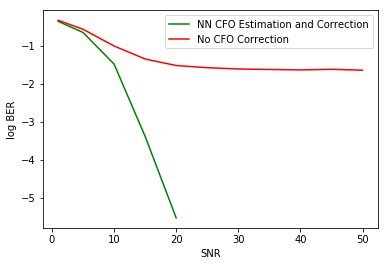
\includegraphics[width=12cm]{figures/cfo/cfo_estimation.png}
\caption{The log BER of received signals passed through a neural network CFO estimator with a rotation matrix CFO correction and classic demodulator. The log BER of the same signals passed through just the classic demodulator.}
\label{fig:cfo_est}
\end{center}
\end{figure}

For SNR above $25$, the neural network does not have any incorrect bits in the $10k$ data sequences each with $100$ symbols, or $50$ bits.  The neural network consistently performs better than just the classic demodulator for all SNR.  Although, the performance is similar for SNR$=1$.


Figure~\ref{fig:cfo_demon_single_tap} shows one example of a data sequence passed through the neural network described above.
The neural network is trained for SNR$=0$. The three plots show that the neural network corrects for CFO quite well.

\setlength{\tabcolsep}{0pt}
\begin{figure}
  \centering
  \caption{Nonlinear neural network estimating and correcting CFO for different $\omega$. In this particular test example, $\omega=0.00969545$ and SNR$=\infty$.}
  \begin{tabular}{ccc}
    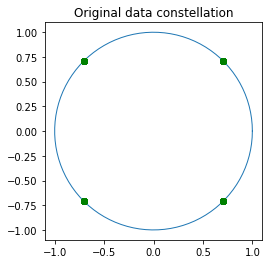
\includegraphics[width=55mm]{figures/cfo/cfo_estimation_original_data.png}&
    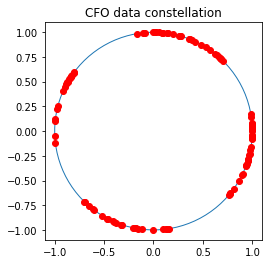
\includegraphics[width=55mm]{figures/cfo/cfo_estimation_cfo_data.png}&
    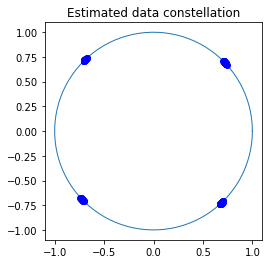
\includegraphics[width=55mm]{figures/cfo/cfo_estimation_est_data.png}\\
  \end{tabular}
  \label{fig:cfo_demon_single_tap}
\end{figure}

In this chapter, we demonstrated that recursive neural networks can act like clocks; they can follow a circle for a given rate of rotation.  They can learn to learn to follow a circle for a given rate.
We have also demonstrated that a neural network can learn to learn how to estimate CFO and correct for it.  All of the simulations in this chapter were for single tap channels.  We attempted to learn how to estimate CFO and correct for it when there were random two tap channels.  However, the results were not promising and will need to be explored more in future work.

%\section{Deep Network Carrier Frequency Offset Correction}
%Program a Costas loop for comparison 